\usetikzlibrary{shapes.geometric}



\tikzset{
itria/.style={
  draw,shape border uses incircle,
  isosceles triangle,shape border rotate=90,yshift=-1.65cm}}
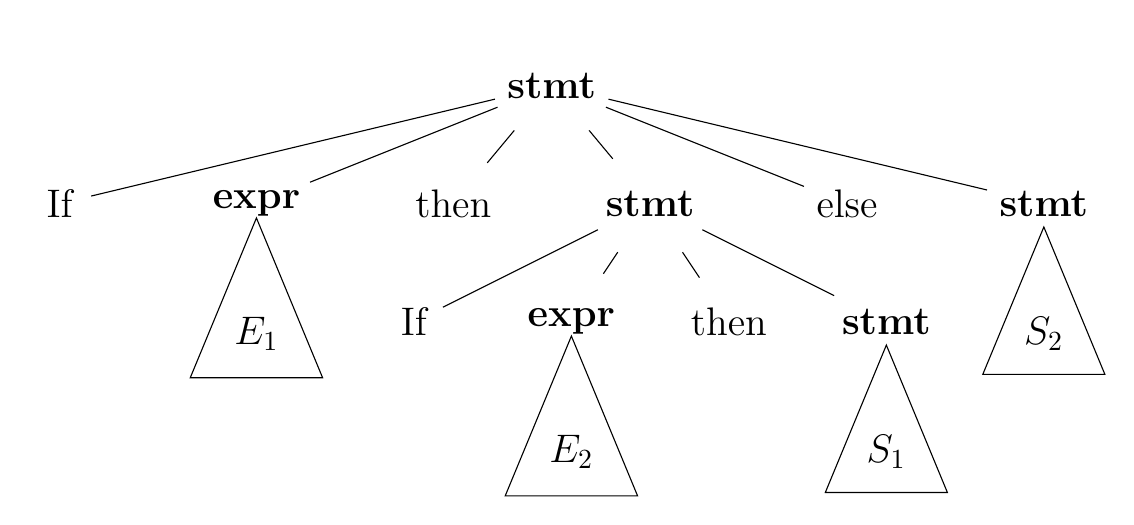
\begin{tikzpicture}[sibling distance=2.5cm, level 2/.style={sibling distance =2cm}]
\node[circle] {\Large{\bf{stmt}}}
 child{ node[circle] {\Large{If}}   }
  child{ node[circle] {\Large{\bf{expr}}}  
     { node[itria] {\Large{$E_1$}} } }
   child{ node[circle] {\Large{then}}   }
    child{ node[circle] {\Large{\bf{stmt}}}
            child{ node[circle] {\Large{If}}
                      %  { node[itria] {Q1} } 
                }
                  child{ node[circle] {\Large{\bf{expr}}}
                       { node[itria] {\Large{$E_2$}} } 
                }
                  child{ node[circle] {\Large{then}}
                      %  { node[itria] {Q1} } 
                }
            child{ node[circle] {\Large{\bf{stmt}}}
                   { node[itria] {\Large{$S_1$}} } 
                }
        }
         child{ node[circle] {\Large{else}}   }
    child{ node[circle] {\Large{\bf{stmt}}}
       { node[itria] {\Large{$S_2$}} } };

\end{tikzpicture}

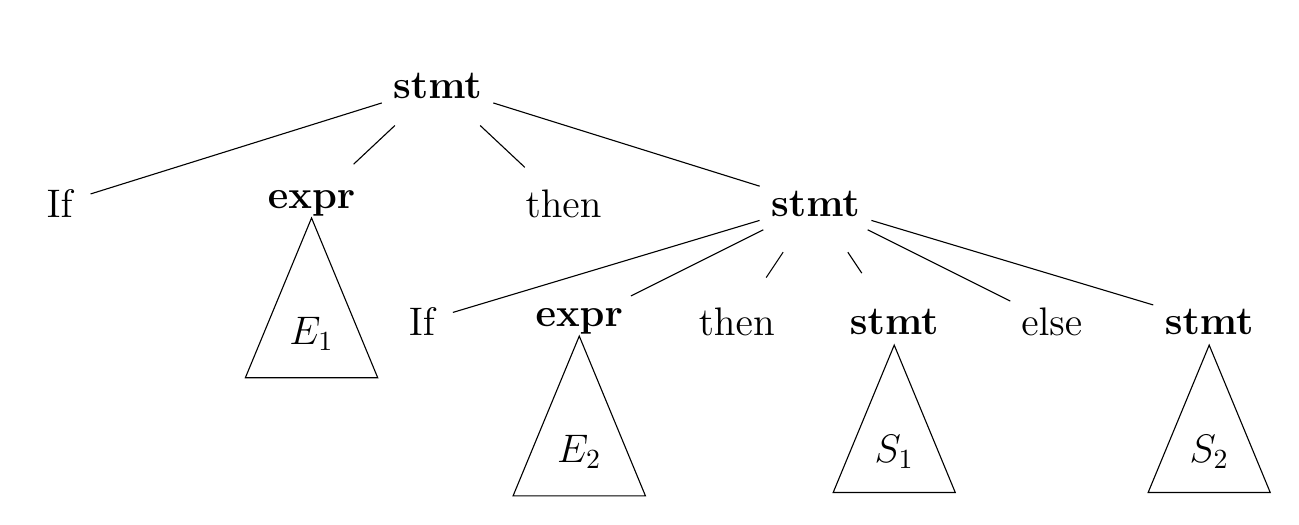
\begin{tikzpicture}[sibling distance=3.2cm, level 2/.style={sibling distance =2cm}]
\node[circle] {\Large{\bf{stmt}}}
 child{ node[circle] {\Large{If}}   }
  child{ node[circle] {\Large{\bf{expr}}}  
     { node[itria] {\Large{$E_1$}} } }
   child{ node[circle] {\Large{then}}   }
    child{ node[circle] {\Large{\bf{stmt}}}
            child{ node[circle] {\Large{If}}
                      %  { node[itria] {Q1} } 
                }
                  child{ node[circle] {\Large{\bf{expr}}}
                       { node[itria] {\Large{$E_2$}} } 
                }
                  child{ node[circle] {\Large{then}}
                      %  { node[itria] {Q1} } 
                }
            child{ node[circle] {\Large{\bf{stmt}}}
                   { node[itria] {\Large{$S_1$}} } 
                }
                   child{ node[circle] {\Large{else}}   }
    child{ node[circle] {\Large{\bf{stmt}}}
       { node[itria] {\Large{$S_2$}} } }
        };

\end{tikzpicture}

%https://gateoverflow.in/3536/gate2007-it-84#35846


\usetikzlibrary{shapes}


\tikzset{pblock/.style = {rectangle split, rectangle split horizontal,
                      rectangle split parts=5, very thick,draw=black!50, align=center}}
                      
\tikzset{qblock/.style = {rectangle split, rectangle split horizontal,
                      rectangle split parts=3, very thick,draw=black!50, align=center}}

\begin{tikzpicture}[]
  \node[pblock,minimum height = 1cm,ultra thick]{\nodepart[text width=0.2mm]{one} 
                \nodepart{two} \Large{K40} \nodepart[text width = 0.2mm]{three} \nodepart[text width = 1cm]{four}  \nodepart[text width = 0.2mm]{five}  };
                
 \node[pblock,minimum height = 1cm,ultra thick] at (-3,-2){\nodepart[text width=0.2mm]{one} 
                \nodepart{two} \Large{K15} \nodepart[text width = 0.2mm]{three} \nodepart{four}\Large{K30}  \nodepart[text width = 0.2mm]{five}  } ;
                
 \node[qblock,minimum height = 1cm,ultra thick] at (7,-2){\nodepart[text width=0.2mm]{one} 
                \nodepart{two} \Large{K50} \nodepart[text width = 0.2mm]{three} \nodepart[text width = 1cm]{four}  \nodepart[text width = 0.2mm]{five}  } ;
                
                
 \node[pblock,minimum height = 1cm,ultra thick] at (-7,-4){\nodepart[text width=0.2mm]{one} 
                \nodepart{two} \Large{K10} \nodepart[text width = 0.2mm]{three} \nodepart[text width = 1cm]{four}  \nodepart[text width = 0.2mm]{five}  };
                
 \node[pblock,minimum height = 1cm,ultra thick] at (-3,-4){\nodepart[text width=0.2mm]{one} 
                \nodepart{two} \Large{K15} \nodepart[text width = 0.2mm]{three} \nodepart{four} \Large{K20}  \nodepart[text width = 0.2mm]{five}  };
                
 \node[pblock,minimum height = 1cm,ultra thick] at (1,-4){\nodepart[text width=0.2mm]{one} 
                \nodepart{two} \Large{K30} \nodepart[text width = 0.2mm]{three} \nodepart[text width = 1cm]{four}  \nodepart[text width = 0.2mm]{five}  };
                
 \node[qblock,minimum height = 1cm,ultra thick] at (5,-4){\nodepart[text width=0.2mm]{one} 
                \nodepart{two} \Large{K40} \nodepart[text width = 0.2mm]{three}   };
                
 \node[qblock,minimum height = 1cm,ultra thick] at (9,-4){\nodepart[text width=0.2mm]{one} 
                \nodepart{two} \Large{K50} \nodepart[text width = 0.2mm]{three}  };
                
                
\draw[*->,thick] (-1.5,0) -- (-1.5,-0.8) -- (-3,-0.8) --(-3,-2);
\draw[*->,thick] (0,0) -- (0,-0.8) -- (6.3,-0.8) --(6.3,-2);

\draw[*->,thick] (7.6,-2.2)  -- (9,-2.2) --(9,-3.7);
\draw[*->,thick] (6.3,-2.2) -- (6.3,-2.2) -- (4.3,-2.2) --(4.3,-4);

\draw[*->,thick] (-3,-2.2) -- (-3,-3.7) ;
\draw[*->,thick] (-4.5,-2.2) -- (-7,-2.2) -- (-7,-3.7);
\draw[*->,thick] (-1.5,-2.2) -- (1,-2.2) -- (1,-3.7);
\end{tikzpicture}

%%%%%%%%%%%%%%%%%%%%%%%%%%%%%%%%%%%%%%%%%%%%%%%%%%%%%%%%%%%%%%%%%%%%%%%%%%%%%%%%%%%%

\begin{tikzpicture}[scale = 0.95,transform shape]
  \node[pblock,minimum height = 1cm,ultra thick]{\nodepart[text width=0.2mm]{one} 
                \nodepart{two} \Large{K20} \nodepart[text width = 0.2mm]{three} \nodepart[text width = 1cm]{four} \Large{K40} \nodepart[text width = 0.2mm]{five}  };
                
 \node[pblock,minimum height = 1cm,ultra thick] at (-5,-2){\nodepart[text width=0.2mm]{one} 
                \nodepart{two} \Large{K15} \nodepart[text width = 0.2mm]{three} \nodepart[text width = 1cm]{four}  \nodepart[text width = 0.2mm]{five}  } ;
                
                 
 \node[pblock,minimum height = 1cm,ultra thick] at (3,-2){\nodepart[text width=0.2mm]{one} 
                \nodepart{two} \Large{K30} \nodepart[text width = 0.2mm]{three} \nodepart[text width = 1cm]{four}  \nodepart[text width = 0.2mm]{five}  } ;               
                
 \node[pblock,minimum height = 1cm,ultra thick] at (11,-2){\nodepart[text width=0.2mm]{one} 
                \nodepart{two} \Large{K50} \nodepart[text width = 0.2mm]{three} \nodepart[text width = 1cm]{four}  \nodepart[text width = 0.2mm]{five}  } ;
                
                
 \node[pblock,minimum height = 1cm,ultra thick] at (-7,-4){\nodepart[text width=0.2mm]{one} 
                \nodepart{two} \Large{K10} \nodepart[text width = 0.2mm]{three} \nodepart[text width = 1cm]{four}  \nodepart[text width = 0.2mm]{five}  };
                
 \node[pblock,minimum height = 1cm,ultra thick] at (-3,-4){\nodepart[text width=0.2mm]{one} 
                \nodepart{two} \Large{K15} \nodepart[text width = 0.2mm]{three} \nodepart[text width = 1cm]{four}   \nodepart[text width = 0.2mm]{five}  };
                
 \node[pblock,minimum height = 1cm,ultra thick] at (1,-4){\nodepart[text width=0.2mm]{one} 
                \nodepart{two} \Large{K20} \nodepart[text width = 0.2mm]{three} \nodepart[text width = 1cm]{four} \Large{K25} \nodepart[text width = 0.2mm]{five}  };
                
 \node[pblock,minimum height = 1cm,ultra thick] at (5,-4){\nodepart[text width=0.2mm]{one} 
                \nodepart{two} \Large{K30} \nodepart[text width = 0.2mm]{three} \nodepart[text width = 1cm]{four}  \nodepart[text width = 0.2mm]{five}  };
                
                
\node[pblock,minimum height = 1cm,ultra thick] at (9,-4){\nodepart[text width=0.2mm]{one} 
                \nodepart{two} \Large{K40} \nodepart[text width = 0.2mm]{three} \nodepart[text width = 1cm]{four}  \nodepart[text width = 0.2mm]{five}  };
                
\node[pblock,minimum height = 1cm,ultra thick] at (15,-4){\nodepart[text width=0.2mm]{one} 
                \nodepart{two} \Large{K50} \nodepart[text width = 0.2mm]{three} \nodepart[text width = 1cm]{four}  \nodepart[text width = 0.2mm]{five}  };
                
                
                
\draw[*->,thick] (-1.5,0) -- (-1.5,-0.8) -- (-5,-0.8) --(-5,-2);
\draw[*->,thick] (0,0) -- (0,-0.8) -- (3,-0.8) --(3,-2);
\draw[*->,thick] (1.5,0) -- (1.5,-0.6) -- (11,-0.6) --(11,-2);

\draw[*->,thick] (9.5,-2) -- (9,-2) --(9,-4);
\draw[*->,thick] (12.5,-2) -- (15,-2) --(15,-4);

\draw[*->,thick] (4.5,-2) -- (5,-2) -- (5,-4);
\draw[*->,thick] (1.5,-2) -- (1,-2) --(1,-4);

\draw[*->,thick] (-6.5,-2) -- (-7,-2) -- (-7,-4);
\draw[*->,thick] (-3.5,-2) -- (-3,-2) --(-3,-4);

%\draw[*->,thick] (6.3,-2.2) -- (6.3,-2.2) -- (4.3,-2.2) --(4.3,-4);

%\draw[*->,thick] (-3,-2.2) -- (-3,-3.7) ;
%\draw[*->,thick] (-4.5,-2.2) -- (-7,-2.2) -- (-7,-3.7);
%\draw[*->,thick] (-1.5,-2.2) -- (1,-2.2) -- (1,-3.7);
\end{tikzpicture}


\usetikzlibrary{shapes}



\tikzset{pblock/.style = {rectangle split, rectangle split horizontal,
                      rectangle split parts=4, very thick,draw=black!80, align=center,ultra thick}}
                      
\tikzset{qblock/.style = {rectangle split, rectangle split horizontal,
                      rectangle split parts=1, very thick,draw=black!80, align=center,ultra thick}}

\tikzset{rblock/.style = {rectangle split, rectangle split horizontal,
                      rectangle split parts=2, very thick,draw=black!80, align=center,ultra thick}}
\tikzset{sblock/.style = {rectangle split, rectangle split horizontal,
                      rectangle split parts=2, very thick,draw=black!80, align=center,ultra thick}}

\begin{tikzpicture}[scale = 0.75,transform shape]
\foreach \y in {0,0.7,1.4,2.1,2.8,3.5}
{
  \node[pblock,minimum height = 0.7cm] at (0,\y){\nodepart[text width=0.5cm]{one} 
                \nodepart[text width=0.5cm]{two}  \nodepart[text width = 9cm]{three} \nodepart[text width = 9cm]{four}  };
                }
                
 \node[pblock,minimum height = 0.7cm,fill=gray!30] at (0,1.4){\nodepart[text width=0.5cm]{one} 
                \nodepart[text width=0.5cm]{two}  \nodepart[text width = 9cm]{three} \nodepart[text width = 9cm]{four}  };
                
\foreach \y in {-7,-7.7,-8.4,-9.1,-9.8,-10.5,-11.2,-11.9,-12.6,-13.3,-14,-14.7,-15.4,-16.1}
{      
\node[qblock,minimum height = 0.7cm] at (6.5,\y){\nodepart[text width=11cm]{one} }; 
 }

\node[qblock,minimum height = 0.7cm,ultra thick,fill=gray!30] at (6.5,-14.7){\nodepart[text width=11cm]{one}}; 

 \foreach \y in {-8.4,-9.1,-9.8,-10.5,-11.2,-11.9}
{      
\node[rblock,minimum height = 0.7cm] at (-5,\y){\nodepart[text width=1cm]{one} \nodepart[text width=5cm]{two} };}

\node[] at (6,5.7){0};  
\node[] at (5.5,5.7){1};  
\node[] at (5,5.7){2};  
\node[] at (4.5,5.7){3};  
 \node[] at (4,5.7){ $\hdots$  }; 
 \node[] at (3.5,5.7){ $\hdots$  }; 
 \node[] at (3,5.7){ $\hdots$  }; 
 \node[] at (2.2,5.7){ 9}; 
 \node[] at (1.7,5.7){ 10  }; 
 \node[] at (1.2,5.7){ 11  }; 
  \node[] at (.7,5.7){ 12  }; 
 \node[] at (.2,5.7){ 13  }; 
  \node[] at (-.4,5.7){ 14  }; 
 \node[] at (-.9,5.7){ 15  }; 
  \node[] at (-1.7,5.7){ $\hdots$  }; 
 \node[] at (-2.2,5.7){ $\hdots$  }; 
  \node[] at (-2.7,5.7){ $\hdots$  }; 
   \node[] at (-3.2,5.7){ $\hdots$  }; 
    \node[] at (-3.7,5.7){ $\hdots$  }; 
    
     \node[] at (-4.2,5.7){ $\hdots$ }; 
      \node[] at (-4.7,5.7){ $\hdots$ }; 
       \node[] at (-5.2,5.7){ 29  }; 
        \node[] at (-5.7,5.7){ 30  }; 
        \node[] at (-6.2,5.7){ 31  };
        
        %%%%%%%%%%%%%%%%%%%%%%%%%%%%%%%%%%%%%%%%%%%%%%%%%
        
        
 \node[rblock,minimum height = 0.7cm,fill=gray!30] at (-5,-9.8){\nodepart[text width=1cm]{one}  \nodepart[text width=5cm]{two}   };
 
\node[sblock,minimum height = 0.7cm] at (0,5){\nodepart[text width= 7cm]{one} \Large{virtual page number} \nodepart[text width= 5cm]{two} \Large{Page Offset}   };  

\node[] at (0,6.5) {\Large{\bf{Virtual Address}}};


\node[sblock,minimum height = 1cm] at (4,-2.5){\nodepart[text width= 6.36cm]{one} \Large{Physical page number} \nodepart[text width= 5cm]{two} \Large{Page Offset}};  
\node[] at (4,-1.8) {\Large{\bf{physical Address}}};

\node[pblock,minimum height = 0.7cm] at (4,-3.5){\nodepart[text width= 5cm]{one} \Large{Physical Address Tag} \nodepart[text width= 3cm]{two} \Large{Cache index} \nodepart[text width= 1.4cm]{three} {Block Offset} \nodepart[text width= 1.4cm]{four} {Byte Offset}    }; 

\node[] at (-9.7,4.1) {Valid};
\node[] at (-8.7,4.1) {dirty};
\node[] at (-4,4.1) {Tag };
\node[] at (5,4.1) {Physical page number};

\node[] at (-7.6,-7.8) {Valid};

\node[] at (-5,-7.8) {Tag};
\node[] at (6.5,-6.3) {\Large{Data}};

\draw[*->,line width = 1mm](6.5,-14.5)-- (6.5,-15.5)  --(6.5,-18) node[below]{\Large{data}};
\draw[->,line width = 1mm](5.5,4.7) -- +(0,-0.3) -- + (6,-0.3) -- +(6,-6) -- +(1.5,-6) -- +(1.5,-6.5);
\draw[*->,line width = 1mm](4.5,1.6) --(4.5,-1.2) -- (.5,-1.2) --(.5,-2);
\draw[->,line width = 1mm] (-5,4.7) -- (-5,0) -- (-5.7,0);
\draw[->,line width=1mm](-5,0.7) --(-5.7,.7);
\draw[->,line width=1mm](-5,1.4) --(-5.7,1.4);
\draw[->,line width=1mm](-5,2.1) --(-5.7,2.1);
\draw[->,line width=1mm](-5,2.8) --(-5.7,2.8);
\draw[->,line width=1mm](-5,3.5) --(-5.7,3.5);

\node[draw,circle,ultra thick] at (-6.3,.7){\bf{=}};
\node[draw,circle,ultra thick] at (-6.3,1.4){\bf{=}};
\node[draw,circle,ultra thick] at (-6.3,2.1){\bf{=}};
\node[draw,circle,ultra thick] at (-6.3,2.8){\bf{=}};
\node[draw,circle,ultra thick] at (-6.3,3.5){\bf{=}};
\node[draw,circle,ultra thick] at (-6.3,0){\bf{=}};


\draw[-] (6.3,-16.7) -- (6.7,-17)node[right]{32};
\draw[-] (11.3,2.7) -- (11.7,3)node[right]{12};
\draw[-] (4.3,-1) -- (4.7,-0.7)node[right]{20};
\draw[-] (8.4,-4.2) -- (8.9,-4.5)node[right]{2};
\draw[-] (7.4,-4.2) -- (7.9,-4.5)node[right]{4};
\draw[-] (5,-4.2) -- (5.4,-4.5)node[right]{8};
\draw[-] (1.9,-4.2) -- (2.4,-4.5)node[right]{18};
\draw[-] (-5.3,4.4) -- (-4.8,4.7)node[right]{20};
\node[circle,fill = black] at (0,-6){};

\draw[->,line width = 1mm](8.7,-4) -- (8.7,-5);
\draw[->,line width = 1mm](7.7,-4) -- (7.7,-6) -- (0.5,-6);
\draw[->,line width = 1mm](5.2,-4) -- (5.2,-5) -- (-8.8,-5) -- (-8.8,-9.8) --(-8.3,-9.8);
\draw[->,line width =1mm] (0,-5) -- (0,-5.8);
\draw[->,line width = 1mm](0,-6.3) -- (0,-14.7) -- (0.5,-14.7);
\draw[-] (-.2,-7.4) -- (.3,-7.7)node[right]{12};

\node[draw,circle,ultra thick] at (-5,-14.7){\bf{=}};

\draw[*->,line width = 1mm] (-5,-9.8) -- (-5,-14.2);
\draw[->,line width = 1mm](2.2,-4) -- (2.2,-4.7) -- (-9.5,-4.7) -- (-9.5,-14.7) --(-5.5,-14.7);

\node[] at (-10.5,-9.8){\Large{cache}};
\node[] at (-11,2.8){\Large{\bf{TLB}}};
\node[] at (-12,2.1){\large{TLB hit}};
\draw[*->,line width = 0.7mm] (-9.7,2.1) -- (-11,2.1);

 \node[and gate US, draw, logic gate inputs=nn, anchor=input 1,rotate = 180,scale=3]
  at
  (-8,-16.7) (and1) {};
  \draw[*-,line width = 0.9mm](-7.5,-9.6) |- (and1.input 2);
  \draw[-,line width= 0.9mm] (-5,-15) |- (and1.input 1);
  \draw[->,line width = 1mm ] (and1.output) -- +(-1,0) node[left]{\large{cache Hit}};

\end{tikzpicture}

 \tikzset{
    rubberduck/.style={
        draw=black!90,
        fill = white,
        shape=isosceles triangle,
        minimum height=5.5cm,
        minimum width=2cm,
        shape border rotate=#1,
        isosceles triangle stretches,
        inner sep=0pt,ultra thick
    },
    rubber/.style={rubberduck=+120},
    ducky/.style={rubberduck=-90}}
 
 
 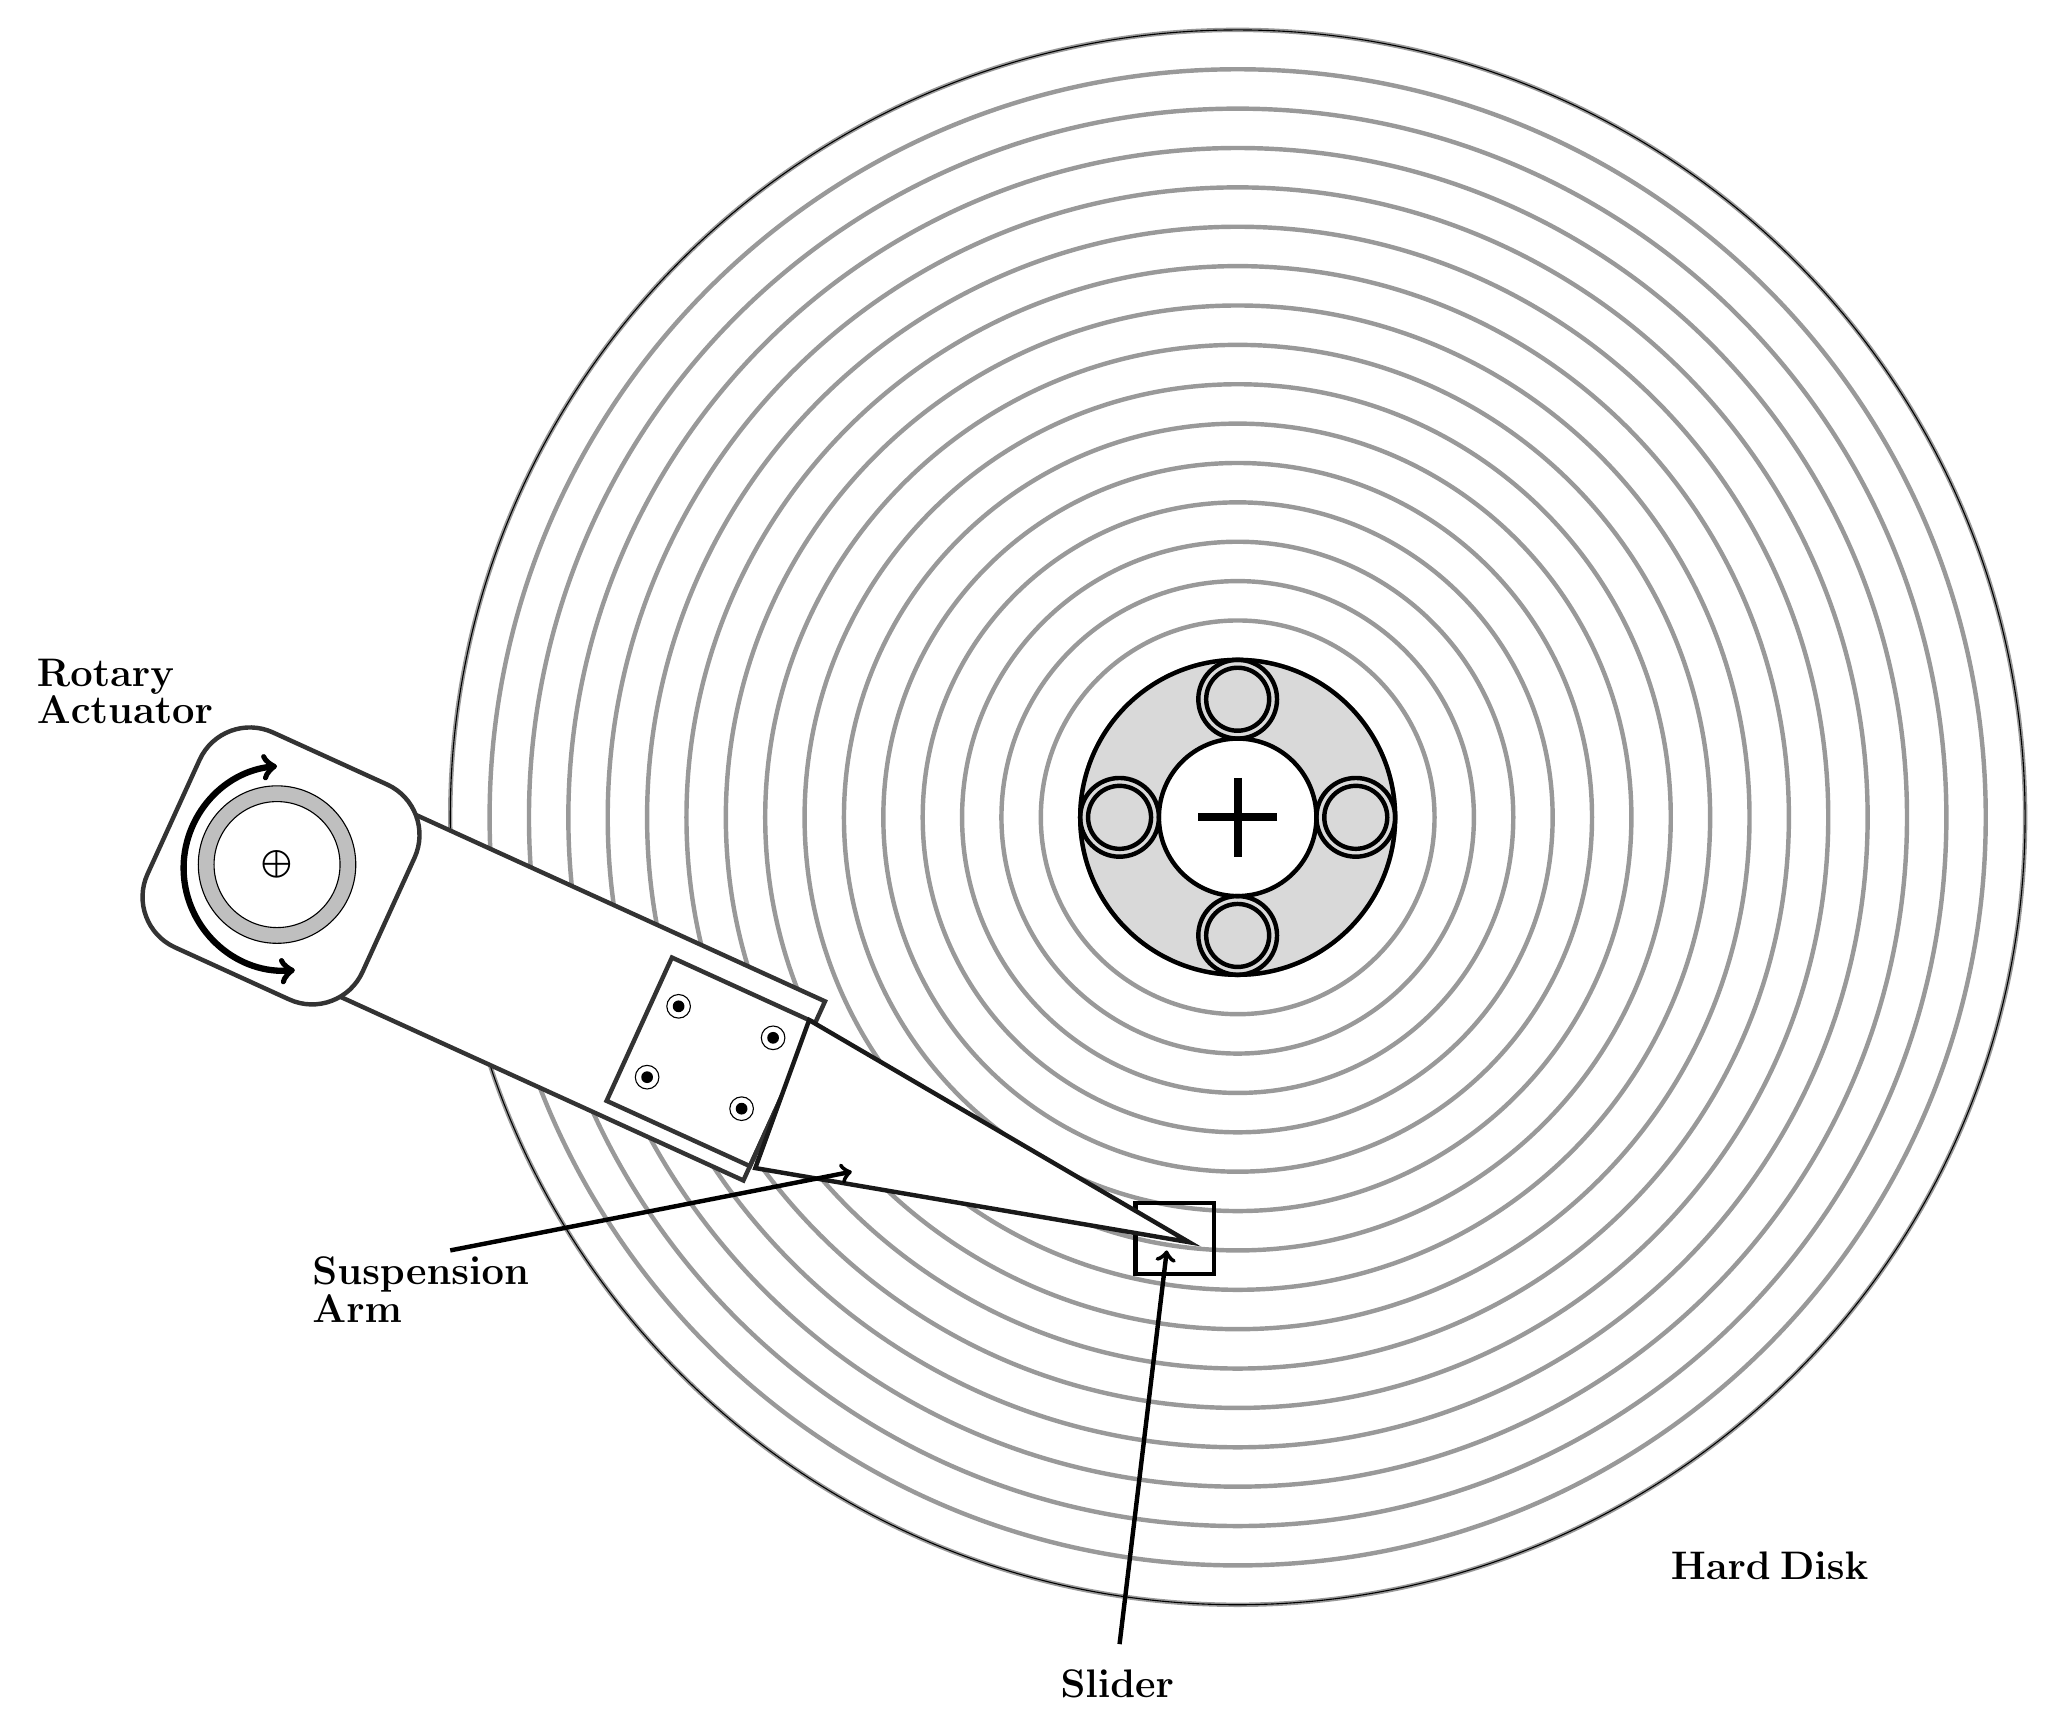
\begin{tikzpicture}
      \foreach \x in {10,20,25,30,35,40,45,50,55,60,65,70,75,80,85,90,95,100}
        \pgfmathsetmacro{\tmp}{0.1*\x}
        \draw[color=black!40,ultra thick] (0,0) circle (\tmp cm); 
        \draw (0,0) node[circle,inner sep=1.5pt,fill,ultra thick] {} circle [radius=10];
        
 
    
 \node[draw,circle,minimum size=4cm,ultra thick,fill = gray!30] at (0,0){};
 \node[draw,circle,minimum size=2cm,ultra thick,fill=white] at (0,0){};
       
       
 \draw[-,line width = 1mm](0,0.5) -- (0,-.5);
           \draw[-,line width = 1mm](0.5,0) -- (-0.5,0);
           
\node[draw,circle,minimum size=1cm,ultra thick] at (-1.5,0){};
\node[draw,circle,minimum size=0.8cm,ultra thick] at (-1.5,0){};
            
\node[draw,circle,minimum size=1cm,ultra thick] at (1.5,0){};
\node[draw,circle,minimum size=0.8cm,ultra thick] at (1.5,0){};
            
 \node[draw,circle,minimum size=1cm,ultra thick] at (0,1.5){};
\node[draw,circle,minimum size=0.8cm,ultra thick] at (0,1.5){};
            
\node[draw,circle,minimum size=1cm,ultra thick] at (0,-1.5){};
\node[draw,circle,minimum size=0.8cm,ultra thick] at (0,-1.5){};
     
\draw[draw=black,ultra thick] (-1.3,-5.8) rectangle ++(1,0.9);

%R2
\draw[draw=black,ultra thick,color = black!80,rotate=-24.5,fill = white] (-9.8,-6.8) rectangle ++(6,2.5);
%R1
\draw[draw=black,ultra thick,color = black!80,rotate=-24.5] (-5.8,-6.6) rectangle ++(2,2);
%rr
\draw[draw=black,ultra thick,color = black!80,rotate=-24.5,rounded corners=20pt,fill=white] (-12.3,-7.1)  rectangle ++(3,3);

     \draw (-6.3,-3.7) node[circle,inner sep=1.5pt,fill,ultra thick] {} circle [radius=0.15];
      \draw (-5.9,-2.8) node[circle,inner sep=1.5pt,fill,ultra thick] {} circle [radius=0.15];
    
\draw (-7.5,-3.3) node[circle,inner sep=1.5pt,fill,ultra thick] {} circle [radius=0.15];
      \draw (-7.1,-2.4) node[circle,inner sep=1.5pt,fill,ultra thick] {} circle [radius=0.15];
        \node[rubber,rotate=-110] at (-5,-3.8){};
   %%%anular   
   \draw[fill=gray!50] (-12.2,-0.6) node[circle,inner sep=1.5pt,fill,ultra thick,] {} circle [radius=1];
\draw[fill=white] (-12.2,-0.6) node[circle,inner sep=1.5pt,ultra thick] {$\bigoplus$} circle [radius=0.8];

\node[text width=2.5cm] at (-14,1.6) {\textbf{\Large{Rotary Actuator}}};
\node[text width=3cm] at (7,-9.5) {\textbf{\Large{Hard Disk}}};

\node[text width=2.5cm] at (-10.5,-6)
{\textbf{\Large{Suspension Arm}}};
\node[text width=2.5cm] at (-1,-11) {\textbf{\Large{Slider}}};
\draw[->,ultra thick] (-1.5,-10.5) -- (-0.9,-5.5);
\draw[->,ultra thick] (-10,-5.5) -- (-4.9,-4.5);
\path [draw=black,rotate=90,<->, ultra thick,line width = 0.8mm ] (0.65,12.2) arc (5:185:1.3cm);
\end{tikzpicture}
